\newpage
\genHeader

\section{Creating instances}

Before diving into modelling dynamic behaviour in Part III, let's have a brief look at how to create a concrete \emph{instance} of your metamodel in Eclipse.

\vspace{0.5cm}

In the following section, we use \emph{metamodel} and \emph{instance} (model) to differentiate between models that represent the abstract syntax and static
semantics of a domain specific language (metamodel), and those that are expressed \emph{in} such a language (instance models of the metamodel).

\begin{itemize}

\item[$\blacktriangleright$] To create an instance model, navigate to the generated \texttt{model} folder in your \texttt{LearningBoxLanguage} project.
Double-click the \texttt{LearningBoxLa\-nguage.ecore} model to invoke  the \emph{Ecore model editor}. 

\vspace{0.5cm}

\item[$\blacktriangleright$] To create a concrete instance of the metamodel, you must select an EClass that will become the root element of the new instance.
For our example, right-click \texttt{Box}, and navigate to ``Create Dynamic Instance'' from the context menu, as depicted in \Cref{fig:context_menu}.

\begin{figure}[htbp]
	\centering
  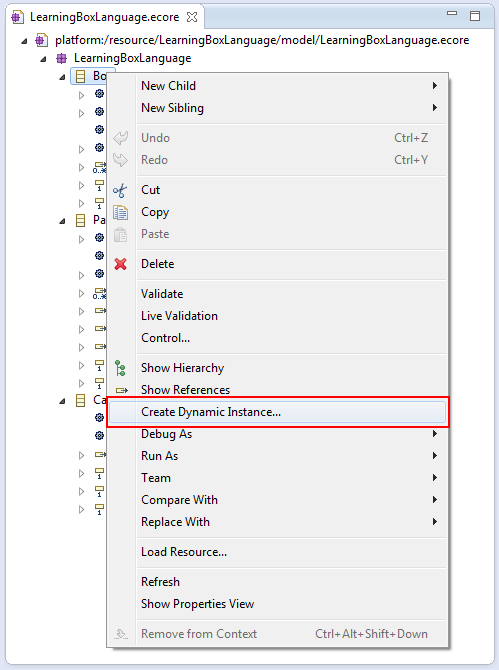
\includegraphics[width=0.6\textwidth]{eclipse_createDynamicInstance}
	\caption{Context menu of an EClass in the Ecore editor}
	\label{fig:context_menu}
\end{figure}

\vspace{0.5cm}

\item[$\blacktriangleright$] A dialogue should appear asking where the instance model file should be persisted. Save your instances according to convention in a
folder named ``instances,'' which is automatically created in every new repository project. Last but not least, enter \texttt{Box.xmi} as the name of the
instance model (\Cref{eclipse:store_dynamic_instance}).

\vspace{0.5cm}

\begin{figure}[htbp]
	\centering
  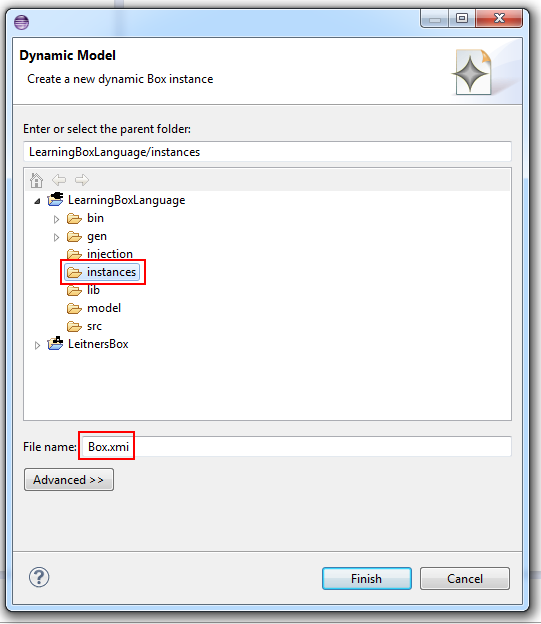
\includegraphics[width=0.6\textwidth]{eclipse_nameDynamicInstance}
	\caption{Dialogue for creating a dynamic model instance}
	\label{eclipse:store_dynamic_instance}
\end{figure}

\item[$\blacktriangleright$] Press \texttt{Finish}, and a generic model editor should open for your new instance model. This editor works just like the
previous Ecore model editor except it's ``generic,'' meaning it allows you to create and edit an instance of \emph{any} metamodel, not only instances of Ecore
(i.e., metamodels).

\clearpage

\item[$\blacktriangleright$] You can populate your instance by adding new children or siblings via a right-click of an element to invoke the
context-menu depicted in \Cref{eclipse:create_instance}. Note that EMF supports you by respecting your metamodel, and reducing the choice of available
elements to valid types only.\footnote{This depends on the current context. Try it out!}

\begin{figure}[htbp]
	\centering
  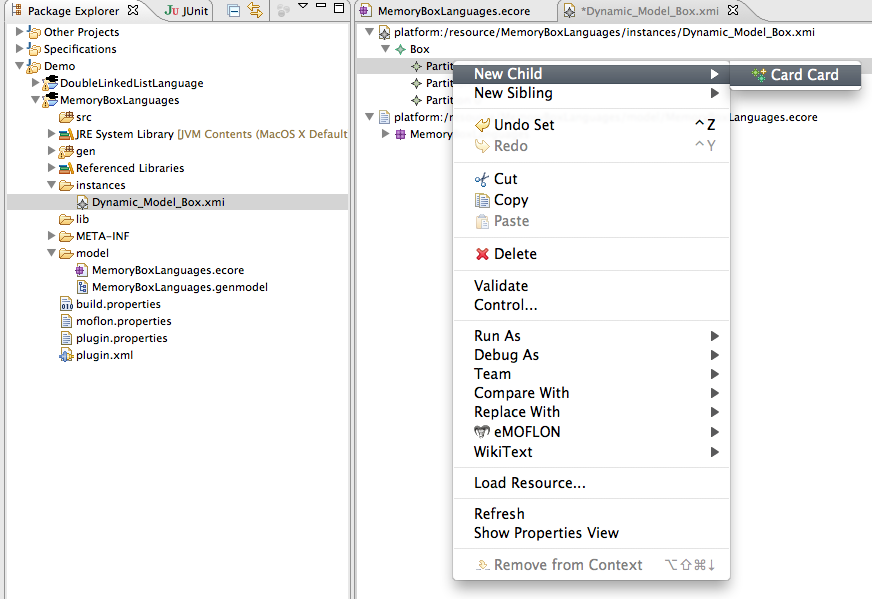
\includegraphics[width=0.8\textwidth]{adjustModel}
	\caption{Context menu for creating model elements}
	\label{eclipse:create_instance}
\end{figure}

\item[$\blacktriangleright$] Let's try building a vocabulary set. Fill your box with three partitions, with two cards in each. Save your model by pressing
\texttt{Ctrl+S} and confirm the save by closing it, then reloading via a simple double-click.

\item[$\blacktriangleright$] Double-click on one of the partitions to bring up the ``Properties'' tab in the window below the editor
(\Cref{eclipse:properties_partition}). Here you'll see the attributes you defined earlier in each EClass. The \texttt{Box}, \texttt{Next}, and
\texttt{Previous} values are its (undefined) EReferences,\footnote{Please note that the editor tab capitilizes the first letter of each property} while \texttt{Index} is a
partition's unique idenfitication value, and \texttt{Partition Size} is the recommended number of cards the partition should contain before being tested.

\begin{figure}[h]
	\centering
  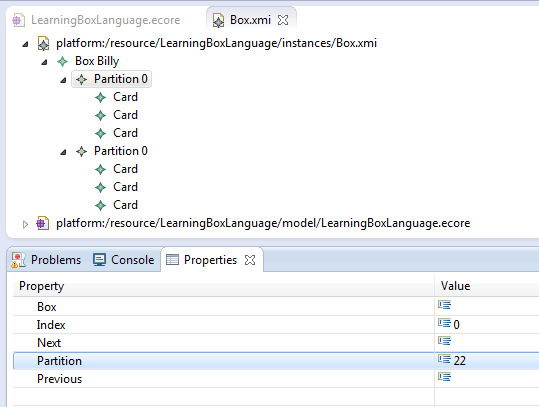
\includegraphics[width=0.6\textwidth]{eclipse_propertiesTab}
	\caption{Change the \texttt{Index} value in the partition's property tab}
	\label{eclipse:properties_partition}
\end{figure}
\FloatBarrier

\vspace{0.5cm}

\item[$\blacktriangleright$] Pick a number - any one you like - and update each partition's \texttt{Index} value. This is their identification value! You'll
notice that as soon as you press \texttt{Enter}, the values will be reflected in the \texttt{.xmi} tree.

\item[$\blacktriangleright$] Now you need to set the \texttt{Next} and \texttt{Previous} EReferences which will make it possible to move cards through the
box. Given that there are no partition before the first, set \texttt{Previous} values only for your second and third partition to that first partition.
Similarly, only set the \texttt{Next} values for the first, and second partition to their respective 'next' partitions.

\item[$\blacktriangleright$] In the same fashion, double click on each \texttt{Card} you created and modify their values. In particular, update the
\texttt{Back} attribute to \texttt{One}. This is the value you'll be able to see from the partition and thus, the \texttt{.xmi} tree. You'll be experimenting
with the \texttt{Face} attribute shortly, so provide a \texttt{1} value for that as well.

\item[$\blacktriangleright$] Fill in the rest the cards with similar vocabulary-style words (such as two/2, three/3, \ldots) that you can `test' yourself on
(\Cref{eclipse:finalXMI}). You now have a unique, customized learning box! Save your model, and ensure no errors exist before proceeding.

\begin{figure}[htbp]
	\centering
  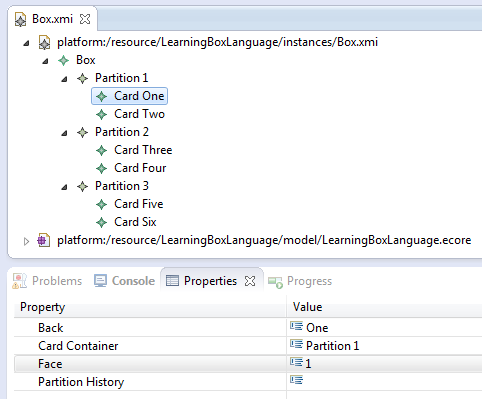
\includegraphics[width=0.7\textwidth]{eclipse_finalBoxXMI}
	\caption{A vocabulary-style learning box}
	\label{eclipse:finalXMI}
\end{figure}

\end{itemize}
